%%%%%%%%%%%%%%%%%%%%%%%%%%%%%%%%%%%%%%%%%%%%%%%%%%%%%%%%%%%%%%%%%%%%%%%%%%

% abnTeX2: Modelo de Trabalho Acadêmico em conformidade com 
% as normas da ABNT

%%%%%%%%%%%%%%%%%%%%%%%%%%%%%%%%%%%%%%%%%%%%%%%%%%%%%%%%%%%%%%%%%%%%%%%%%%

\documentclass[english, 
brazil, 
bsc] 
%Opções msist = Mapeamento Sistemático
{ftec-abntex2}


%%%%%%%%%%%%%%%%%%%%%%%%%%%%%%%%%%%%%%%%%%%%%%%%%%%%%%%%%%%%%%%%%%%%%%%%%%
% Área para adição de pacotes extras
%%%%%%%%%%%%%%%%%%%%%%%%%%%%%%%%%%%%%%%%%%%%%%%%%%%%%%%%%%%%%%%%%%%%%%%%%%

\usepackage{lipsum} %Retirar para a versão final do documento

%Utilize aqui seu pacote preferido para algoritmos
\usepackage[linesnumbered]{algorithm2e}

%%%%%%%%%%%%%%%%%%%%%%%%%%%%%%%%%%%%%%%%%%%%%%%%%%%%%%%%%%%%%%%%%%%%%%%%%%

%Compila o indice
\makeindex

\begin{document}
	
	% Seleciona o idioma do documento (conforme pacotes do babel)
	\selectlanguage{brazil}
	
	% Retira espaço extra obsoleto entre as frases.
	\frenchspacing 
	
	%%%%%%%%%%%%%%%%%%%%%%%%%%%%%%%%%%%%%%%%%%%%%%%%%%%%%%%%%%%%%%%%%%%%%%%%%%
	% ELEMENTOS PRÉ-TEXTUAIS
	%%%%%%%%%%%%%%%%%%%%%%%%%%%%%%%%%%%%%%%%%%%%%%%%%%%%%%%%%%%%%%%%%%%%%%%%%%
	
	\pretextual
	
	\titulo{ChatGPT: Uma análise da ferramenta aplicada no processo de desenvolvimento de software} 
	\autor{Victor Junio Lisboa Costa}
	\orientador{Prof. Msc Lucilia Ribeiro}
	\curso{Ciência da Computação}
	
	\inserirInformacoesPDF
	
	\imprimircapa
	\imprimirfolhaderosto*
	
	\imprimirfolhadeaprovacao
	
	\begin{dedicatoria}
   \vspace*{\fill}
   \centering
   \noindent
   \textit{Este trabalho é dedicado a todos que desejam se concentrar mais no conteúdo de seus trabalhos e menos nas normas de formatação.} \vspace*{\fill}
\end{dedicatoria}
% ---
	\begin{agradecimentos}

\lipsum[1-4]

\end{agradecimentos}
% ---
	\begin{epigrafe}[]
    \vspace*{\fill}
	\begin{flushright}
	
		\textit{Este trabalho, além de cultural, filosófico e pedagógico\\
				É também medicinal, preventivo e curativo\\
				Servindo entre outras coisas para pano branco e pano preto\\
				Curuba e ferida braba\\
				Piolho, chulé e caspa\\
				Cravo, espinha e berruga\\
				Panarismo e água na pleura\\
				Só não cura o velho chifre\\
				Por que não mata a raiz\\
				Pois fica ela encravada\\
				No fundo do coração\\
				(Falcão)}
		
	\end{flushright}
\end{epigrafe}
% ---
	% resumo em português
\setlength{\absparsep}{18pt} % ajusta o espaçamento dos parágrafos do resumo
\begin{resumo}
 
Segundo a \citeonline[3.1-3.2]{NBR6028:2003}, o resumo deve ressaltar o objetivo, o método, os resultados e as conclusões do documento. A ordem e a extensão destes itens dependem do tipo de resumo (informativo ou indicativo) e do tratamento que cada item recebe no documento original. O resumo deve ser precedido da referência do documento, com exceção do resumo inserido no próprio documento. (\ldots) As palavras-chave devem figurar logo abaixo do resumo, antecedidas da expressão Palavras-chave:, separadas entre si por ponto e finalizadas também por ponto.

 \textbf{Palavras-chave}: latex. abntex. editoração de texto.
\end{resumo}
	% resumo em inglês
\setlength{\absparsep}{18pt} % ajusta o espaçamento dos parágrafos do resumo
\begin{resumo}[Abstract]
 \begin{otherlanguage*}{english}
   This is the english abstract.

   \vspace{\onelineskip}
 
   \noindent 
   \textbf{Keywords}: latex. abntex. text editoration.
 \end{otherlanguage*}
\end{resumo}
	
	
	\mostrarlistadeILUSTRACOES
	%\mostrarlistadeQUADROS
	\mostrarlistadeTABELAS
	%\mostrarlistadeCODIGOS
	%\mostrarlistadeALGORITMOS
	
	% Lista de abreviaturas e siglas

\begin{siglas}
	\item[ABNT]{Associação Brasileira de Normas Técnicas}
	\item[abnTeX]{ABsurdas Normas para TeX}
	\item[FTEC]{FACULDADE DE TECNOLOGIA TECBRASIL}
\end{siglas}
	% ---
% inserir lista de símbolos
% ---

\begin{simbolos}
  \item[$ \Gamma $] Letra grega Gama
  \item[$ \Lambda $] Lambda
  \item[$ \zeta $] Letra grega minúscula zeta
  \item[$ \in $] Pertence
\end{simbolos}
% ---
	
	\mostrarSUMARIO
	
	%%%%%%%%%%%%%%%%%%%%%%%%%%%%%%%%%%%%%%%%%%%%%%%%%%%%%%%%%%%%%%%%%%%%%%%%%%
	% ELEMENTOS TEXTUAIS
	%%%%%%%%%%%%%%%%%%%%%%%%%%%%%%%%%%%%%%%%%%%%%%%%%%%%%%%%%%%%%%%%%%%%%%%%%%
	
	\textual
	\chapter{Introdução}

Este documento e seu código-fonte são exemplos de referência de uso da classe \textbf{abntex2} e do pacote \textbf{abntex2cite}. O documento exemplifica a elaboração de trabalho acadêmico (tese, dissertação e outros do gênero) produzido conforme a ABNT NBR 14724:2011 \emph{Informação e documentação - Trabalhos acadêmicos - Apresentação}.

A expressão ``Modelo Canônico'' é utilizada para indicar que \abnTeX\ não é modelo específico de nenhuma universidade ou instituição, mas que implementa tão somente os requisitos das normas da ABNT. Uma lista completa das normas observadas pelo \abnTeX\ é apresentada em \citeonline{abntex2classe}.

Sinta-se convidado a participar do projeto \abnTeX! Acesse o site do projeto em \url{http://www.abntex.net.br/}. Também fique livre para conhecer, estudar, alterar e redistribuir o trabalho do \abnTeX, desde que os arquivos modificados tenham seus nomes alterados e que os créditos sejam dados aos autores originais, nos termos da ``The \LaTeX\ Project Public License''\footnote{\url{http://www.latex-project.org/lppl.txt}}.

Encorajamos que sejam realizadas customizações específicas deste exemplo para universidades e outras instituições --- como capas, folha de aprovação, etc. Porém, recomendamos que ao invés de se alterar diretamente os arquivos do \abnTeX, distribua-se arquivos com as respectivas customizações. Isso permite que futuras versões do \abnTeX~não se tornem automaticamente incompatíveis com as customizações promovidas. Consulte \citeonline{abntex2-wiki-como-customizar} para mais informações.

Este documento deve ser utilizado como complemento dos manuais do \abnTeX\ \cite{abntex2classe,abntex2cite,abntex2cite-alf} e da classe \textsf{memoir} \cite{memoir}. 

Esperamos, sinceramente, que o \abnTeX\ aprimore a qualidade do trabalho que você produzirá, de modo que o principal esforço seja concentrado no principal: na contribuição científica. 

Equipe \abnTeX. 

Lauro César Araujo
	\chapter{Fundamentação Teórica}

	\include{Conteudo/03_FundamentacaoTeorica}
	\chapter{Metodologia}

Breve descrição das próximas subseções...

\subsection{Questões de pesquisa}

Descrição de todas as perguntas que se pretende responder ao final deste trabalho... 

A seguir as questões de pesquisa:
\begin{enumerate}
	\item Questão de pesquisa 01;
	\item Questão de pesquisa 02;
	\item Questão de pesquisa 03;
	\item Questão de pesquisa 04;
	\item Questão de pesquisa n.
\end{enumerate}

\subsection{Estratégia de busca}

Descrição das estratégias de busca, informando as bases e as strings utilizadas...

Foram utilizadas as seguintes bases de pesquisa:
\begin{itemize}
	\item BASE \url{<https://base-search.net/about/en/index.php>};
	\item ERIC	\url{<https://eric.ed.gov/>};
	\item IEEE Xplore Digital Library	\url{<http://ieeexplore.ieee.org>};
	\item SciELO	\url{<https://search.scielo.org/>};
	\item Science Direct	\url{<https://www.sciencedirect.com/>}.
\end{itemize}


Na Tabela \ref{palavra_chave} são apresentadas as Palavras-Chave utilizadas utilizadas para formar a \textit{string} de busca.
Para auxiliar na criação de tabelas pode-se utilizar o site \url{https://www.tablesgenerator.com/}

\begin{table}[ht]
	\centering
	\label{palavra_chave}
	\caption{Palavras-Chave utilizadas na \textit{string} de busca}
	\begin{tabular}{|c|c|}
		\hline
		\textbf{\begin{tabular}[c]{@{}c@{}}Palavra chave\end{tabular}}                             & \textbf{\begin{tabular}[c]{@{}c@{}}Sinônimo em Inglês\end{tabular}} \\ \hline
		café                                                                                           & Coffee, cafe                                                            \\ \hline
		\begin{tabular}[c]{@{}c@{}}máquina (Referente a cafeteira ou máquina de café)\end{tabular} & machine, make, maker                                                    \\ \hline
		portátil                                                                                       & portable, mini, hand, tiny                                              \\ \hline
	\end{tabular}
\end{table}



Na Tabela \ref{string} é apresentada a \textit{string} utilizada para as buscas nas bases:

\begin{table}[h!]
	\centering
	\label{string}
	\caption{ \textit{String} utilizada para realizar as buscas nas bases}
	\begin{tabular}{|l|}
		\hline
		\textbf{\begin{tabular}[c]{@{}l@{}}( ( coffee  OR  cafe )  AND  ( machine  OR  make  OR  maker )\\   AND   ( portable  OR  mini  OR  hand  OR  tiny ) )\end{tabular}} \\ \hline
	\end{tabular}
\end{table}


A seguir os Critérios de Inclusão:
\begin{enumerate}
	\item Critério 01;
	\item Critério 02;
	\item Critério 03;
	\item Critério 04;
	\item Critério n.
\end{enumerate}


A seguir os Critérios de Exclusão:
\begin{enumerate}
	\item Critério 01;
	\item Critério 02;
	\item Critério 03;
	\item Critério 04;
	\item Critério n.
\end{enumerate}

	\chapter{Apresentação e Análise de Resultados}

Breve descrição das próximas subseções...\\

Descrever a estratégia utilizada para ler os artigos. EX.: primeiro título, depois palavras-chave, resumo, conclusão, ...
Descrição das atividades realizadas na subseções...\\
Obs.: Inclua Figuras, Tabelas, Quadros, Códigos, etc...

\begin{figure}[htb]
	\caption{\label{fig:criterios}Fluxo de extração dos estudos}   
	\begin{center}
		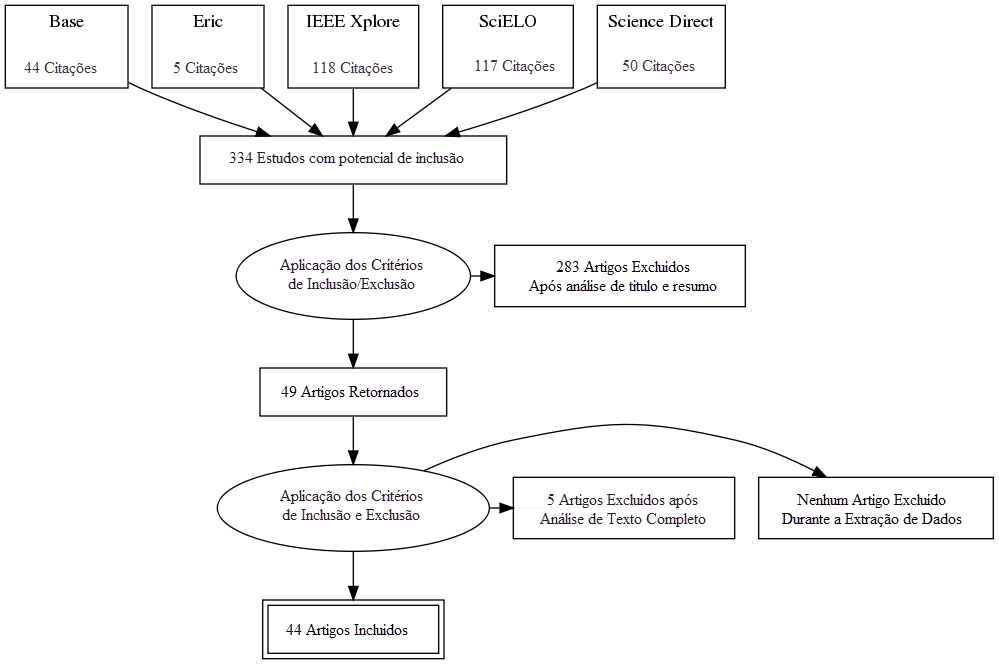
\includegraphics[scale=0.7]{Imagens/EstrategiadeBusca.dot.png}
	\end{center}
	\legend{Fonte: Elaborada pela autora}
\end{figure}

A Figura \ref{fig:criterios} apresenta um fluxo descrevendo o processo de extração dos artigos desde a base até a análise. Pode utilizar o site \url{http://prisma.thetacollaborative.ca/} para gerar automaticamente.


	\chapter{Considerações Finais}

Descrição das atividades realizadas para atingir o objetivo do trabalho... 2 paragrafos \\
Descrição da metodologia utilizada para atingir o objetivo do trabalho... 1 paragrafo \\
Descrição dos pontos fracos ou que possam inviabilizar a credibilidade do trabalho... 1 paragrafo \\
Descrição das atividades futuras para se concluir o trabalho... 1 paragrafo
	
	\phantompart
	\bibliography{Referencias}
	
	%%%%%%%%%%%%%%%%%%%%%%%%%%%%%%%%%%%%%%%%%%%%%%%%%%%%%%%%%%%%%%%%%%%%%%%%%%
	% ELEMENTOS PÓS-TEXTUAIS
	%%%%%%%%%%%%%%%%%%%%%%%%%%%%%%%%%%%%%%%%%%%%%%%%%%%%%%%%%%%%%%%%%%%%%%%%%%
	
	%\postextual
	
	%\renewcommand{\chapnumfont}{\chaptitlefont}
	%\renewcommand{\afterchapternum}{}
	%\begin{apendicesenv}

% Imprime uma página indicando o início dos apêndices
\partapendices

% ----------------------------------------------------------
\chapter{Quisque libero justo}
% ----------------------------------------------------------

\lipsum[50]

% ----------------------------------------------------------
\chapter{Nullam elementum urna vel imperdiet sodales elit ipsum pharetra ligula
ac pretium ante justo a nulla curabitur tristique arcu eu metus}
% ----------------------------------------------------------
\lipsum[55-57]

\end{apendicesenv}

	%\begin{anexosenv}


% Imprime uma página indicando o início dos anexos
\partanexos

% ---
\chapter{Morbi ultrices rutrum lorem.}
% ---
\lipsum[30]

% ---
\chapter{Cras non urna sed feugiat cum sociis natoque penatibus et magnis dis
parturient montes nascetur ridiculus mus}
% ---

\lipsum[31]

% ---
\chapter{Fusce facilisis lacinia dui}
% ---

\lipsum[32]


\end{anexosenv}

	
\end{document}
